%% LyX 2.0.6 created this file.  For more info, see http://www.lyx.org/.
%% Do not edit unless you really know what you are doing.
\documentclass[12pt,spanish]{article}
\usepackage{fontspec}
\usepackage[landscape,paperwidth=60cm,paperheight=40cm]{geometry}
\geometry{verbose,tmargin=2.5cm,bmargin=3cm,lmargin=3cm,rmargin=3cm}
\setlength{\parindent}{0bp}
\usepackage{graphicx}
\usepackage[numbers]{natbib}

\makeatletter
%%%%%%%%%%%%%%%%%%%%%%%%%%%%%% Textclass specific LaTeX commands.
\usepackage{enumitem}		% customizable list environments
\newlength{\lyxlabelwidth}      % auxiliary length 

%%%%%%%%%%%%%%%%%%%%%%%%%%%%%% User specified LaTeX commands.
\usepackage{multicol}

\makeatother

\usepackage{xunicode}
\usepackage{polyglossia}
\setdefaultlanguage{spanish}
\begin{document}
\large


\title{\Huge{Navarro-Frenk-White en Simulaciones Cosmologicas Usando MCMC}}


\author{\huge{Christian Poveda}}


\date{\LARGE{Universidad de los Andes}}

\maketitle
\setlength{\columnsep}{1.5cm}
\begin{multicols}{3}
\thispagestyle{empty}




\section{Introducción}


\subsection{Perfil de Navarro-Frenk-White }

El perfil de Navarro-Frenk-White permite obtener la densidad de materia
oscura de un halo en función del radio y está dado por
\[
\rho\left(R;\rho_{0},R_{s}\right)=\frac{\rho_{0}}{\frac{R}{R_{s}}\left(1+\frac{R}{R_{s}}\right)^{2}}
\]
Integrando es posible obtener la masa contenida en función del radio
\[
M\left(R;\rho_{0},R_{s}\right)=4\pi\rho_{0}R_{s}^{3}\left[\log\left(1+\frac{R}{R_{s}}\right)-\frac{R}{R_{s}+R}\right]
\]
Adicionalmente se suele definir el radio virial de un halo $R_{vir}$
como el valor de $r$ tal que $\left\langle \rho\right\rangle \left(R_{vir}\right)=n\rho_{back}$
donde $n$ es el factor de sobredensidad y la concentración de cada
halo como $c:=R_{vir}/R_{s}$ \citep{NFW}. Así se puede normalizar
el perfil de masa 
\[
m\left(r;c\right)=A\left[\log\left(1+rc\right)-\frac{rc}{1+rc}\right]
\]
Donde $r=R/R_{vir}$ y
\[
A=\left[\log\left(1+c\right)-\frac{c}{1+c}\right]^{-1}
\]
A continuación se muestra la masa normalizada con distintos valores
de la concentración 

\begin{center}
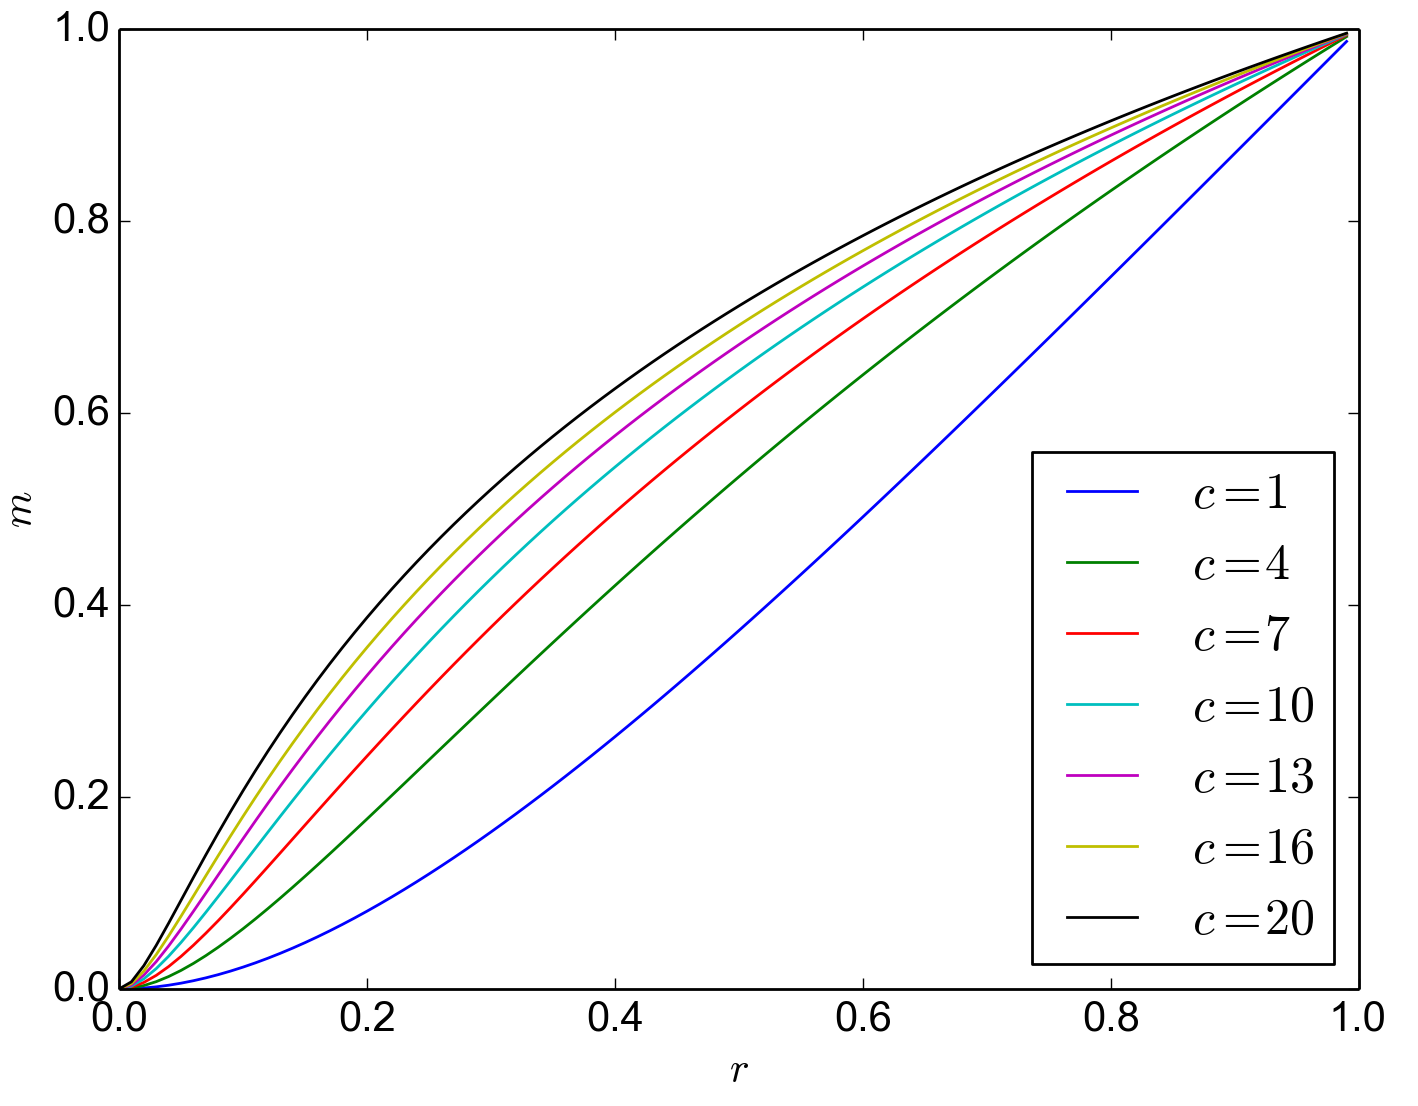
\includegraphics[scale=0.6]{conc}
\par\end{center}


\subsection{Friend-Of-Friend}

Fue inventado en 1985 por Davis et al.\citep{FOF}. Este algoritmo
buscador de halos consiste en definir una longitud de enlace a partír
de un umbral de densidad. Si dos partículas están separadas por una
distancia menor a su longitud de enlace, pertenecen al mismo halo.

\begin{center}
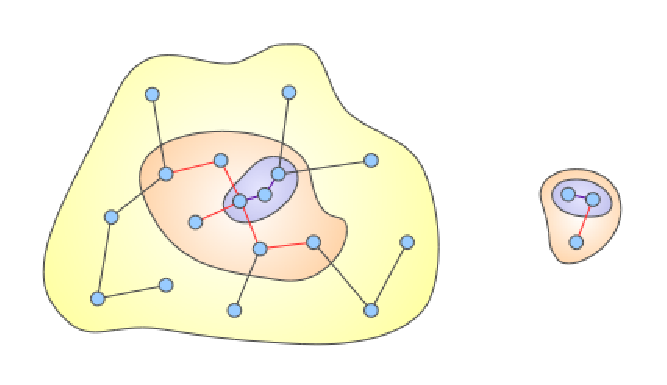
\includegraphics[scale=0.9]{FOFgroups-sub-linklength}
\par\end{center}


\subsection{Bound Density Maximum}

Fue inventado en 1997 por Klypin y Holtzman \citep{BDM}. Consiste
en buscar máximos locales de densidad, luego se recorta el halo donde
sea lo suficientemente denso ($r_{vir}$) y se remueven las partículas
que no estén ligadas. En MultiDark hay dos catálogos: BDMV ($\eta=360$)
y BDMW ($\eta=740$).

\begin{center}
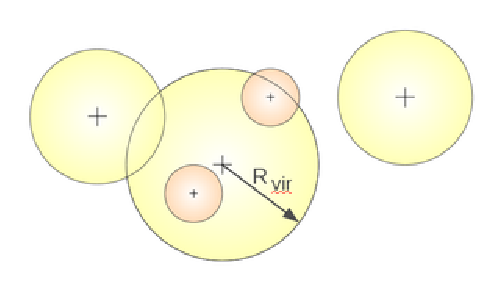
\includegraphics[scale=0.9]{BDMhalos-s}
\par\end{center}


\section{Muestreando con MCMC}


\subsection{Definiendo un Centro}

Se toma el centro de cada halo como su mínimo de potencial

\[
\phi\left(\vec{R}_{i}\right)=-\sum_{j\neq i}\frac{Gm^{2}}{\left\Vert \vec{R}_{i}-\vec{R}_{j}\right\Vert }
\]


Luego se redefinen las coordenadas de cada partícula respecto a este
nuevo centro

\[
\vec{R}_{i}^{\prime}=\vec{R}_{i}-\vec{R}_{c}
\]


Se cuenta el número de partículas dentro de cada radio. Despues de
esto se calcula el radio virial, se eliminan las partículas con un
radio mayor a este y se normalizan las distancias. En la siguiente
gráfica se muestra la proyección de un halo deÑ catálogo FOF-MDR1
sobre el plano y-z con sus respectivos radios viriales

\begin{center}
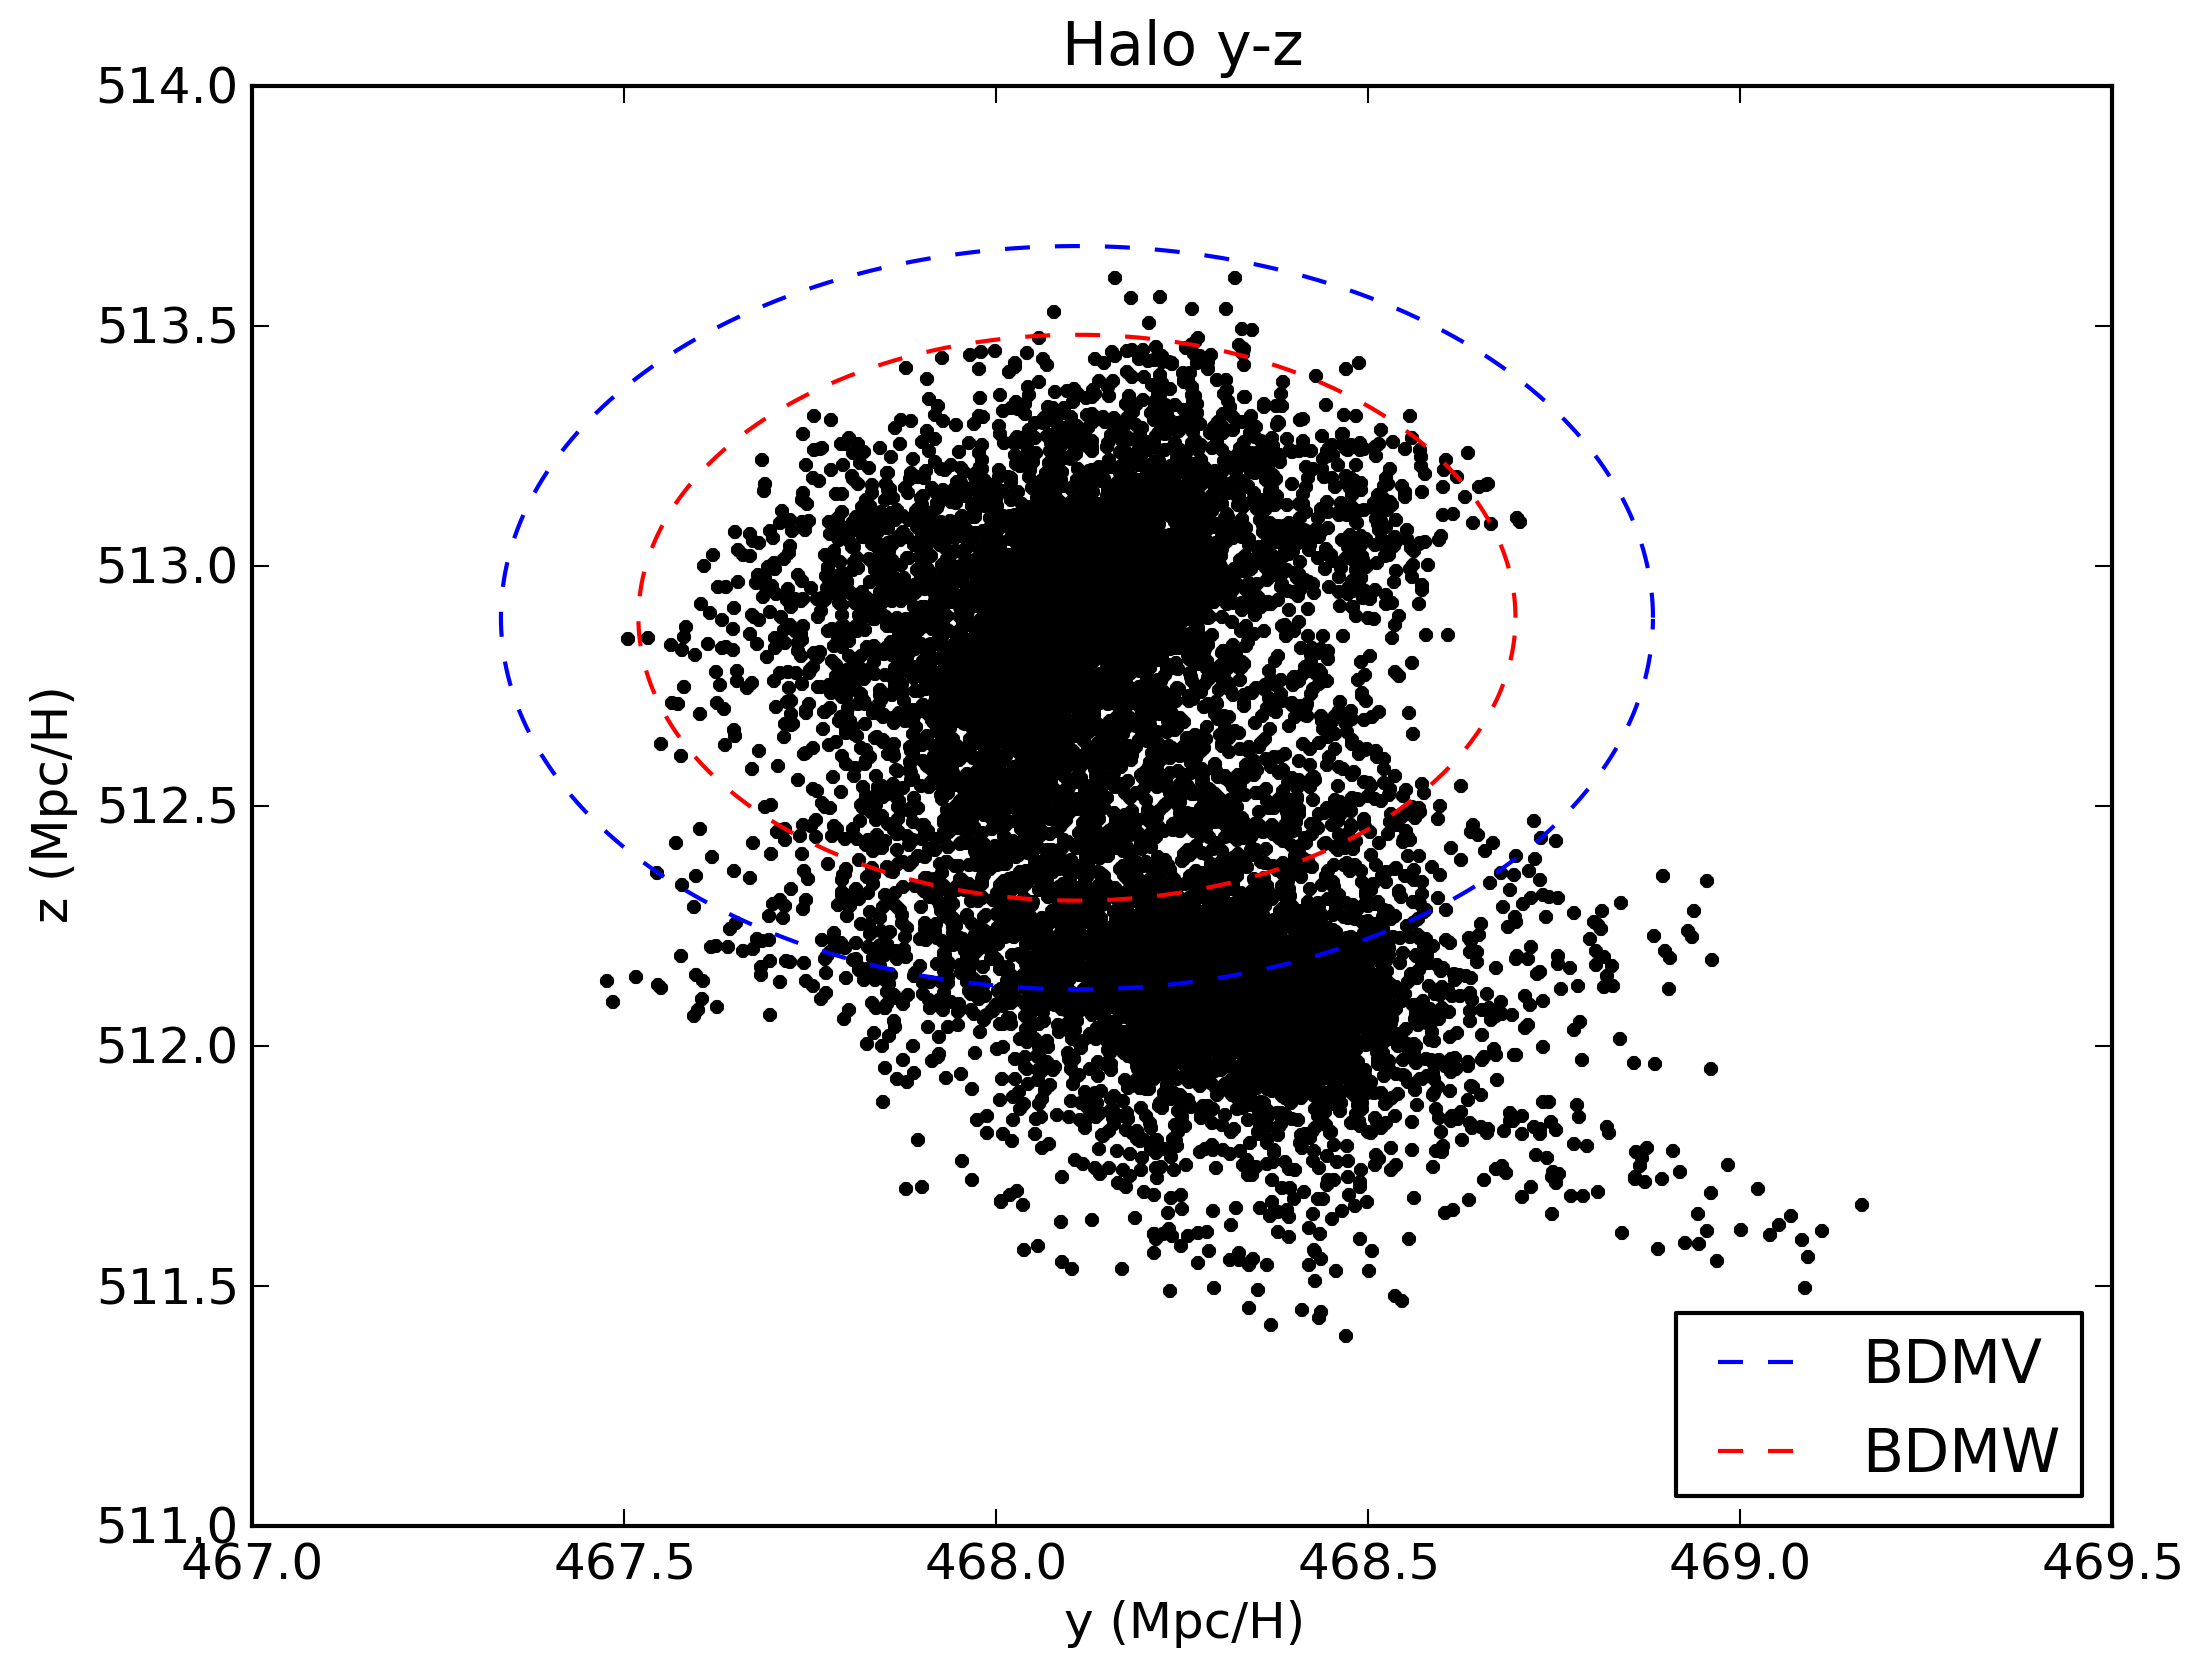
\includegraphics[scale=0.6]{halo_yz}
\par\end{center}


\subsection{Algoritmo de Metropolis-Hastings }

Se utiliza el algoritmo de Metropolis-Hastings para muestrear la verosimilitud

\[
{\cal L}\left(c\right)=\exp\left(-\chi^{2}\left(c\right)\right)
\]


\[
\chi^{2}\left(c\right)=\sum_{i}\left(m_{i}-m_{NFW}\left(r_{i};c\right)\right)^{2}
\]


Luego se toma el valor de donde ${\cal L}\left(c\right)$ es máxima,
sin embargo se toma la reestricción $c\geq1$. Para el halo mostrado
anteriormente vemos que

\begin{center}
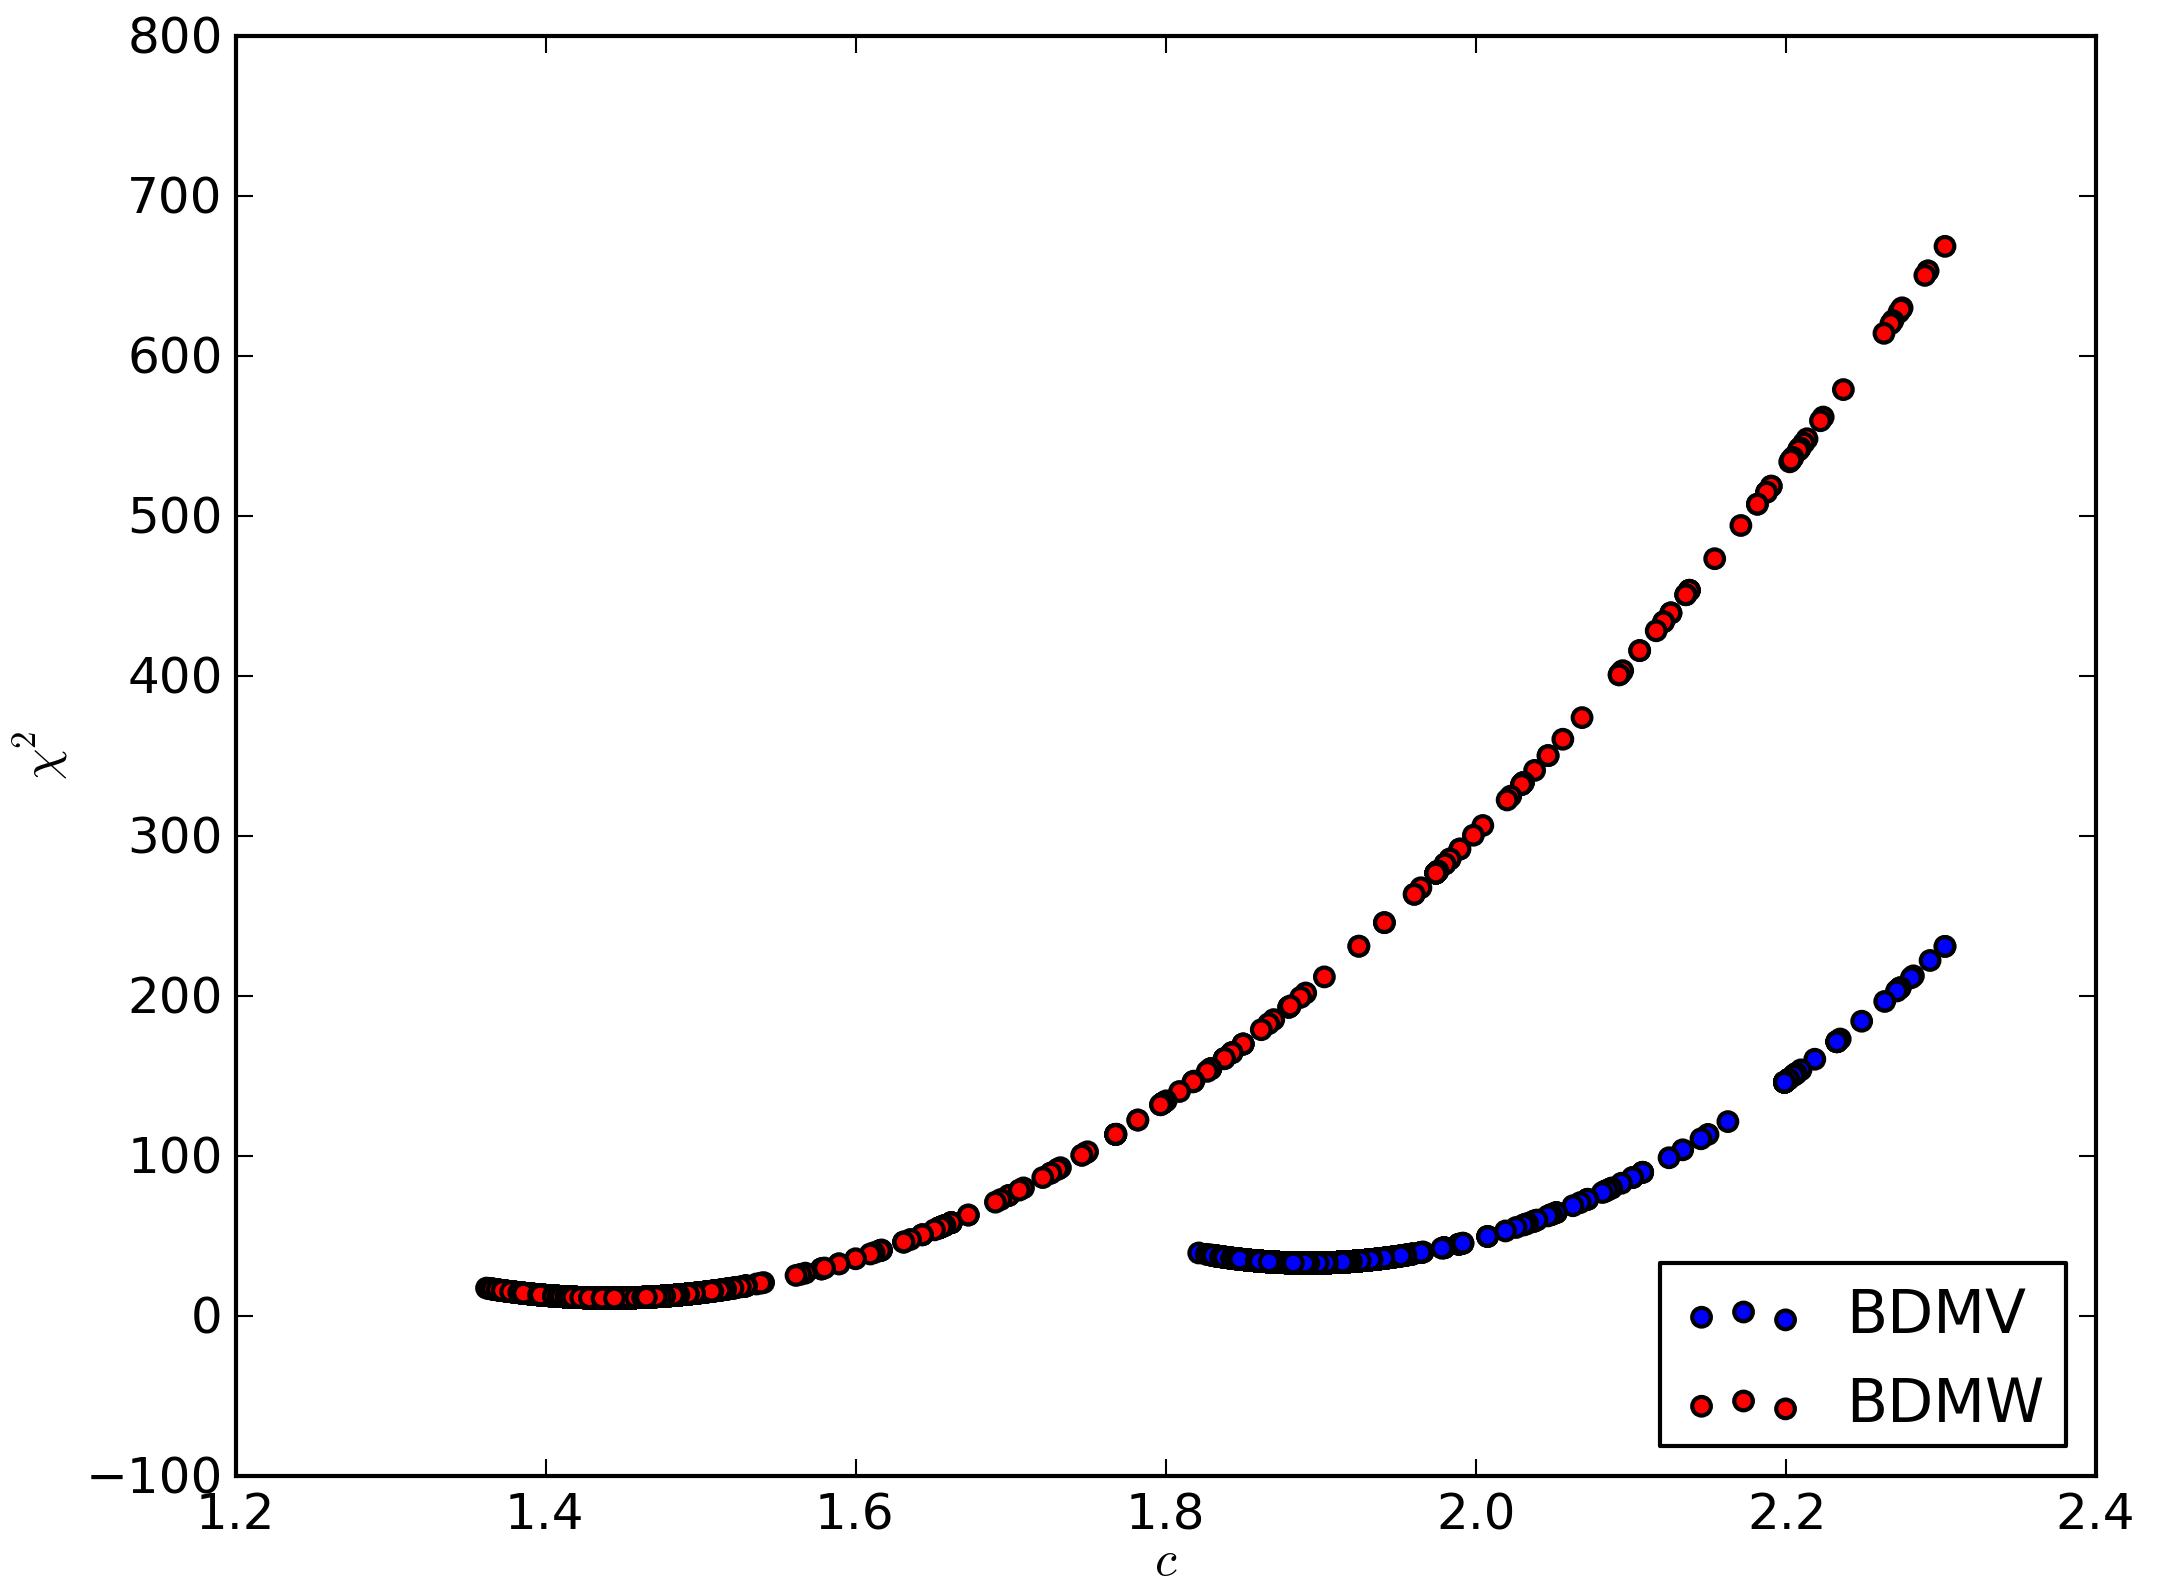
\includegraphics[scale=0.6]{chi2}
\par\end{center}

Tomando el valor de $c$ que corresponde al mínimo valor de $\chi^{2}$
para ambos casos, se obtienen las siguientes curvas

\begin{center}
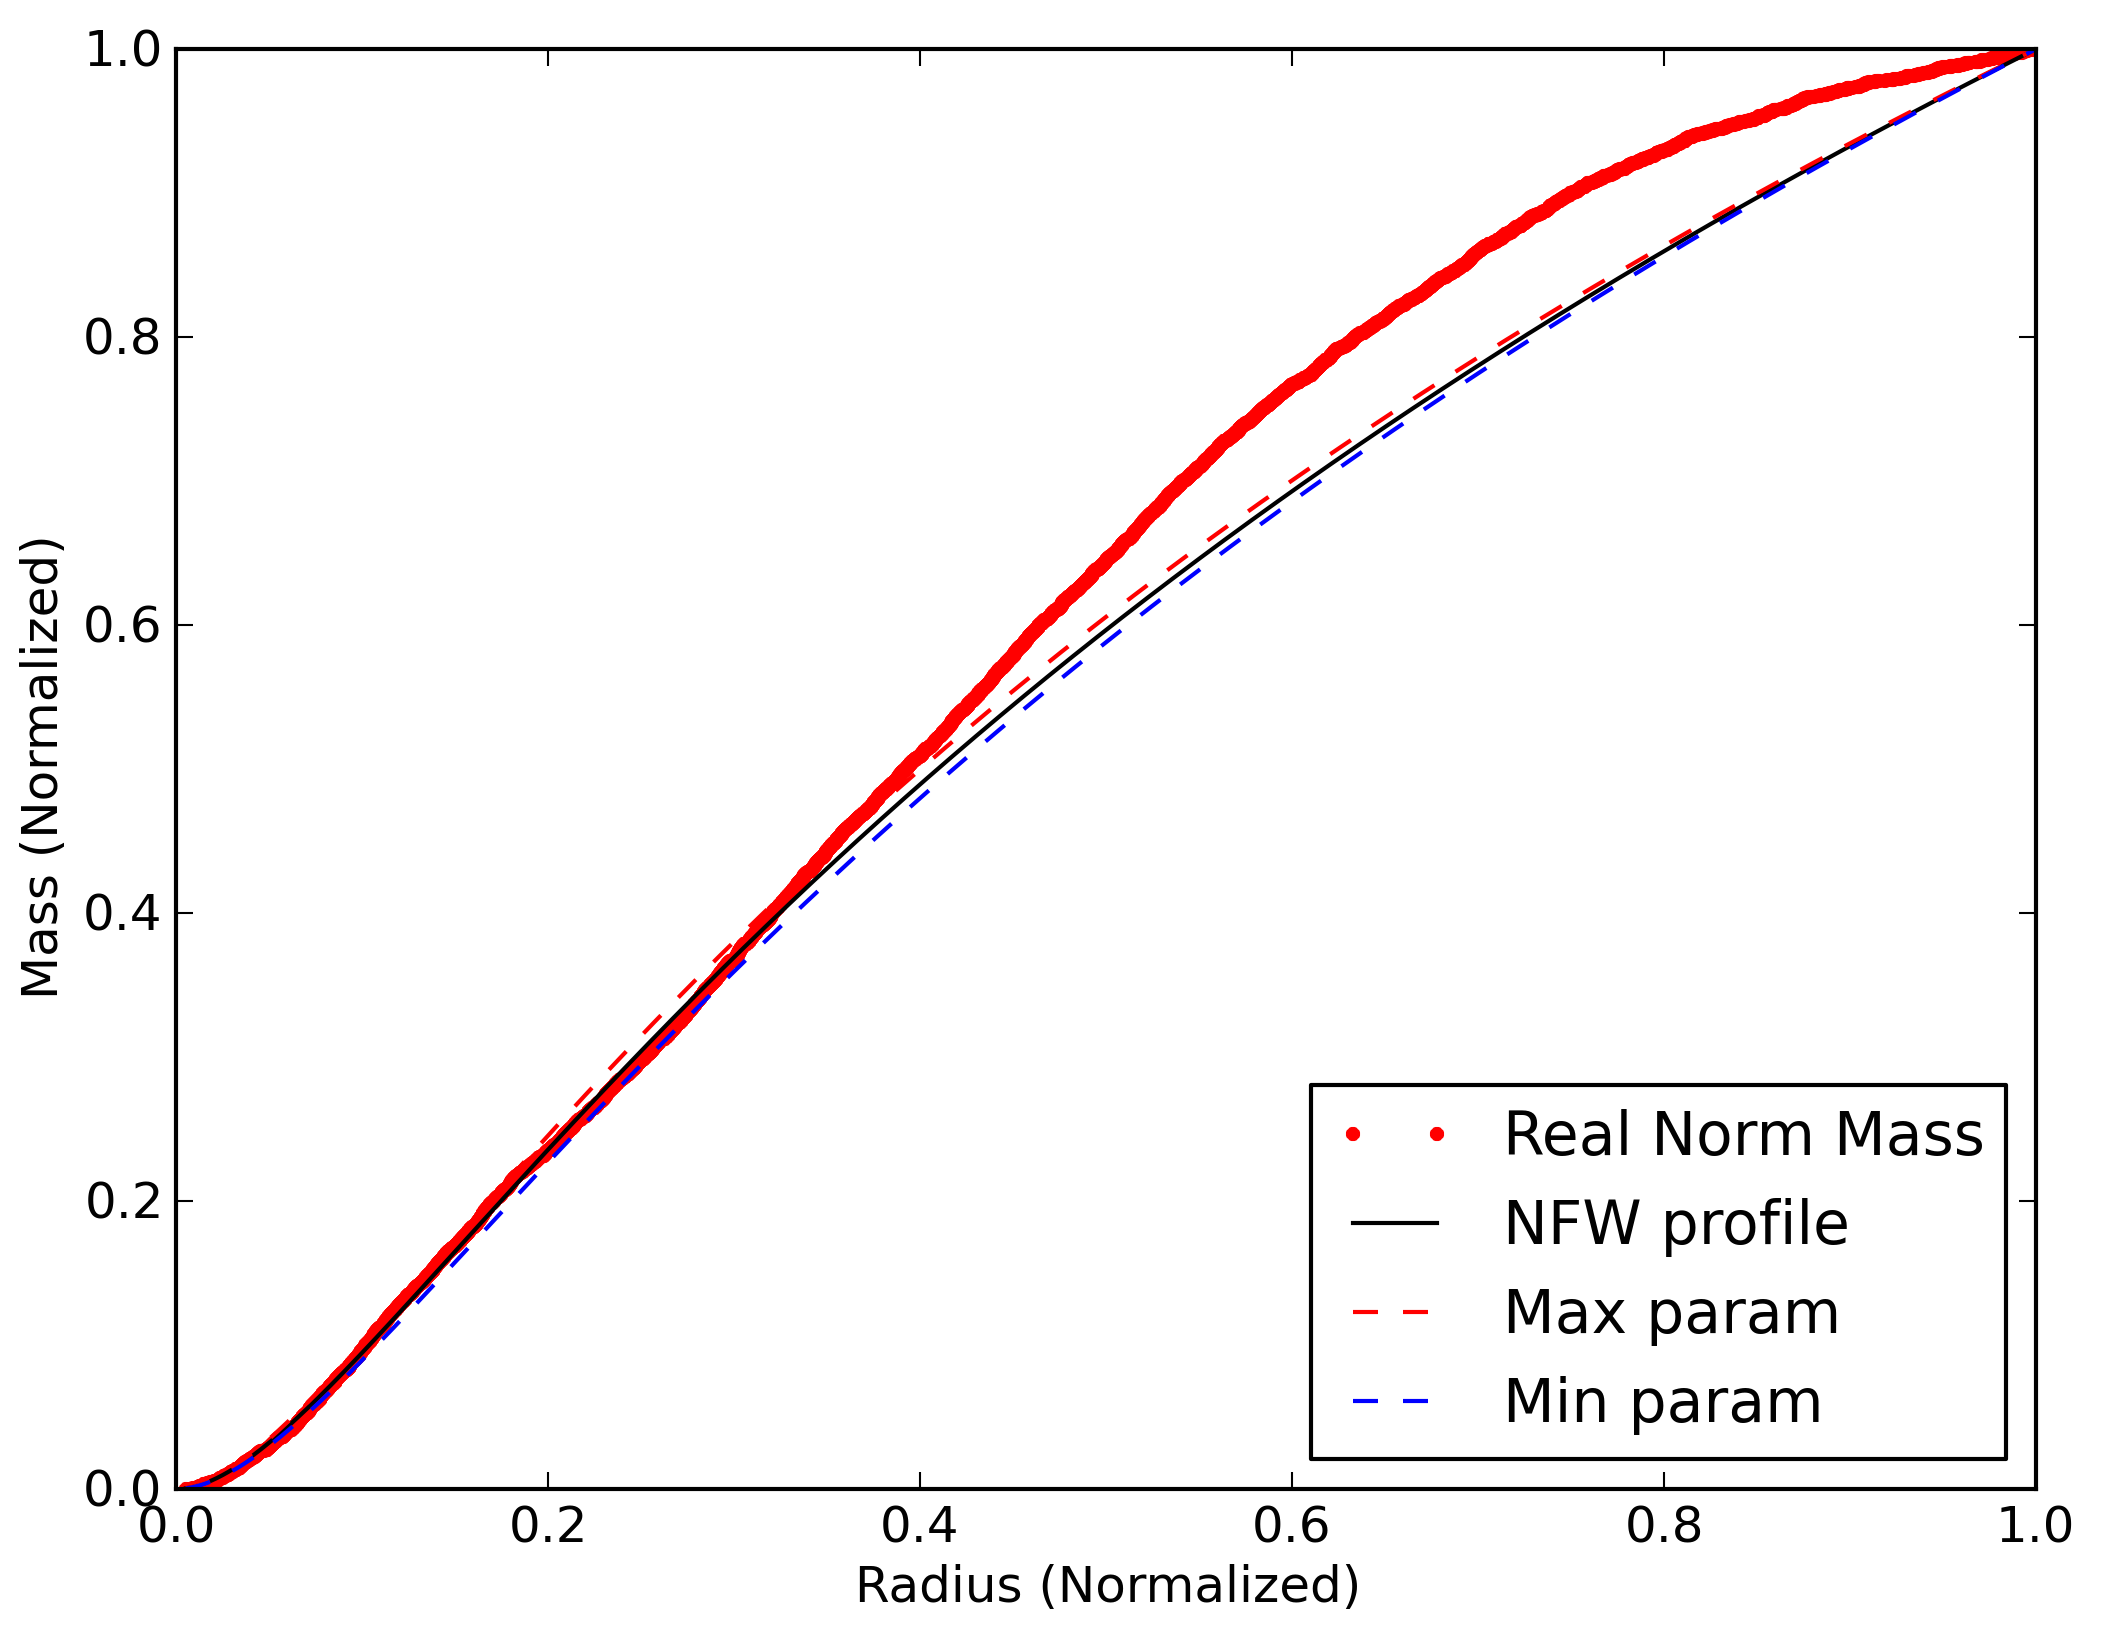
\includegraphics[scale=0.6]{mass_norm_BDMV}
\par\end{center}

\begin{center}
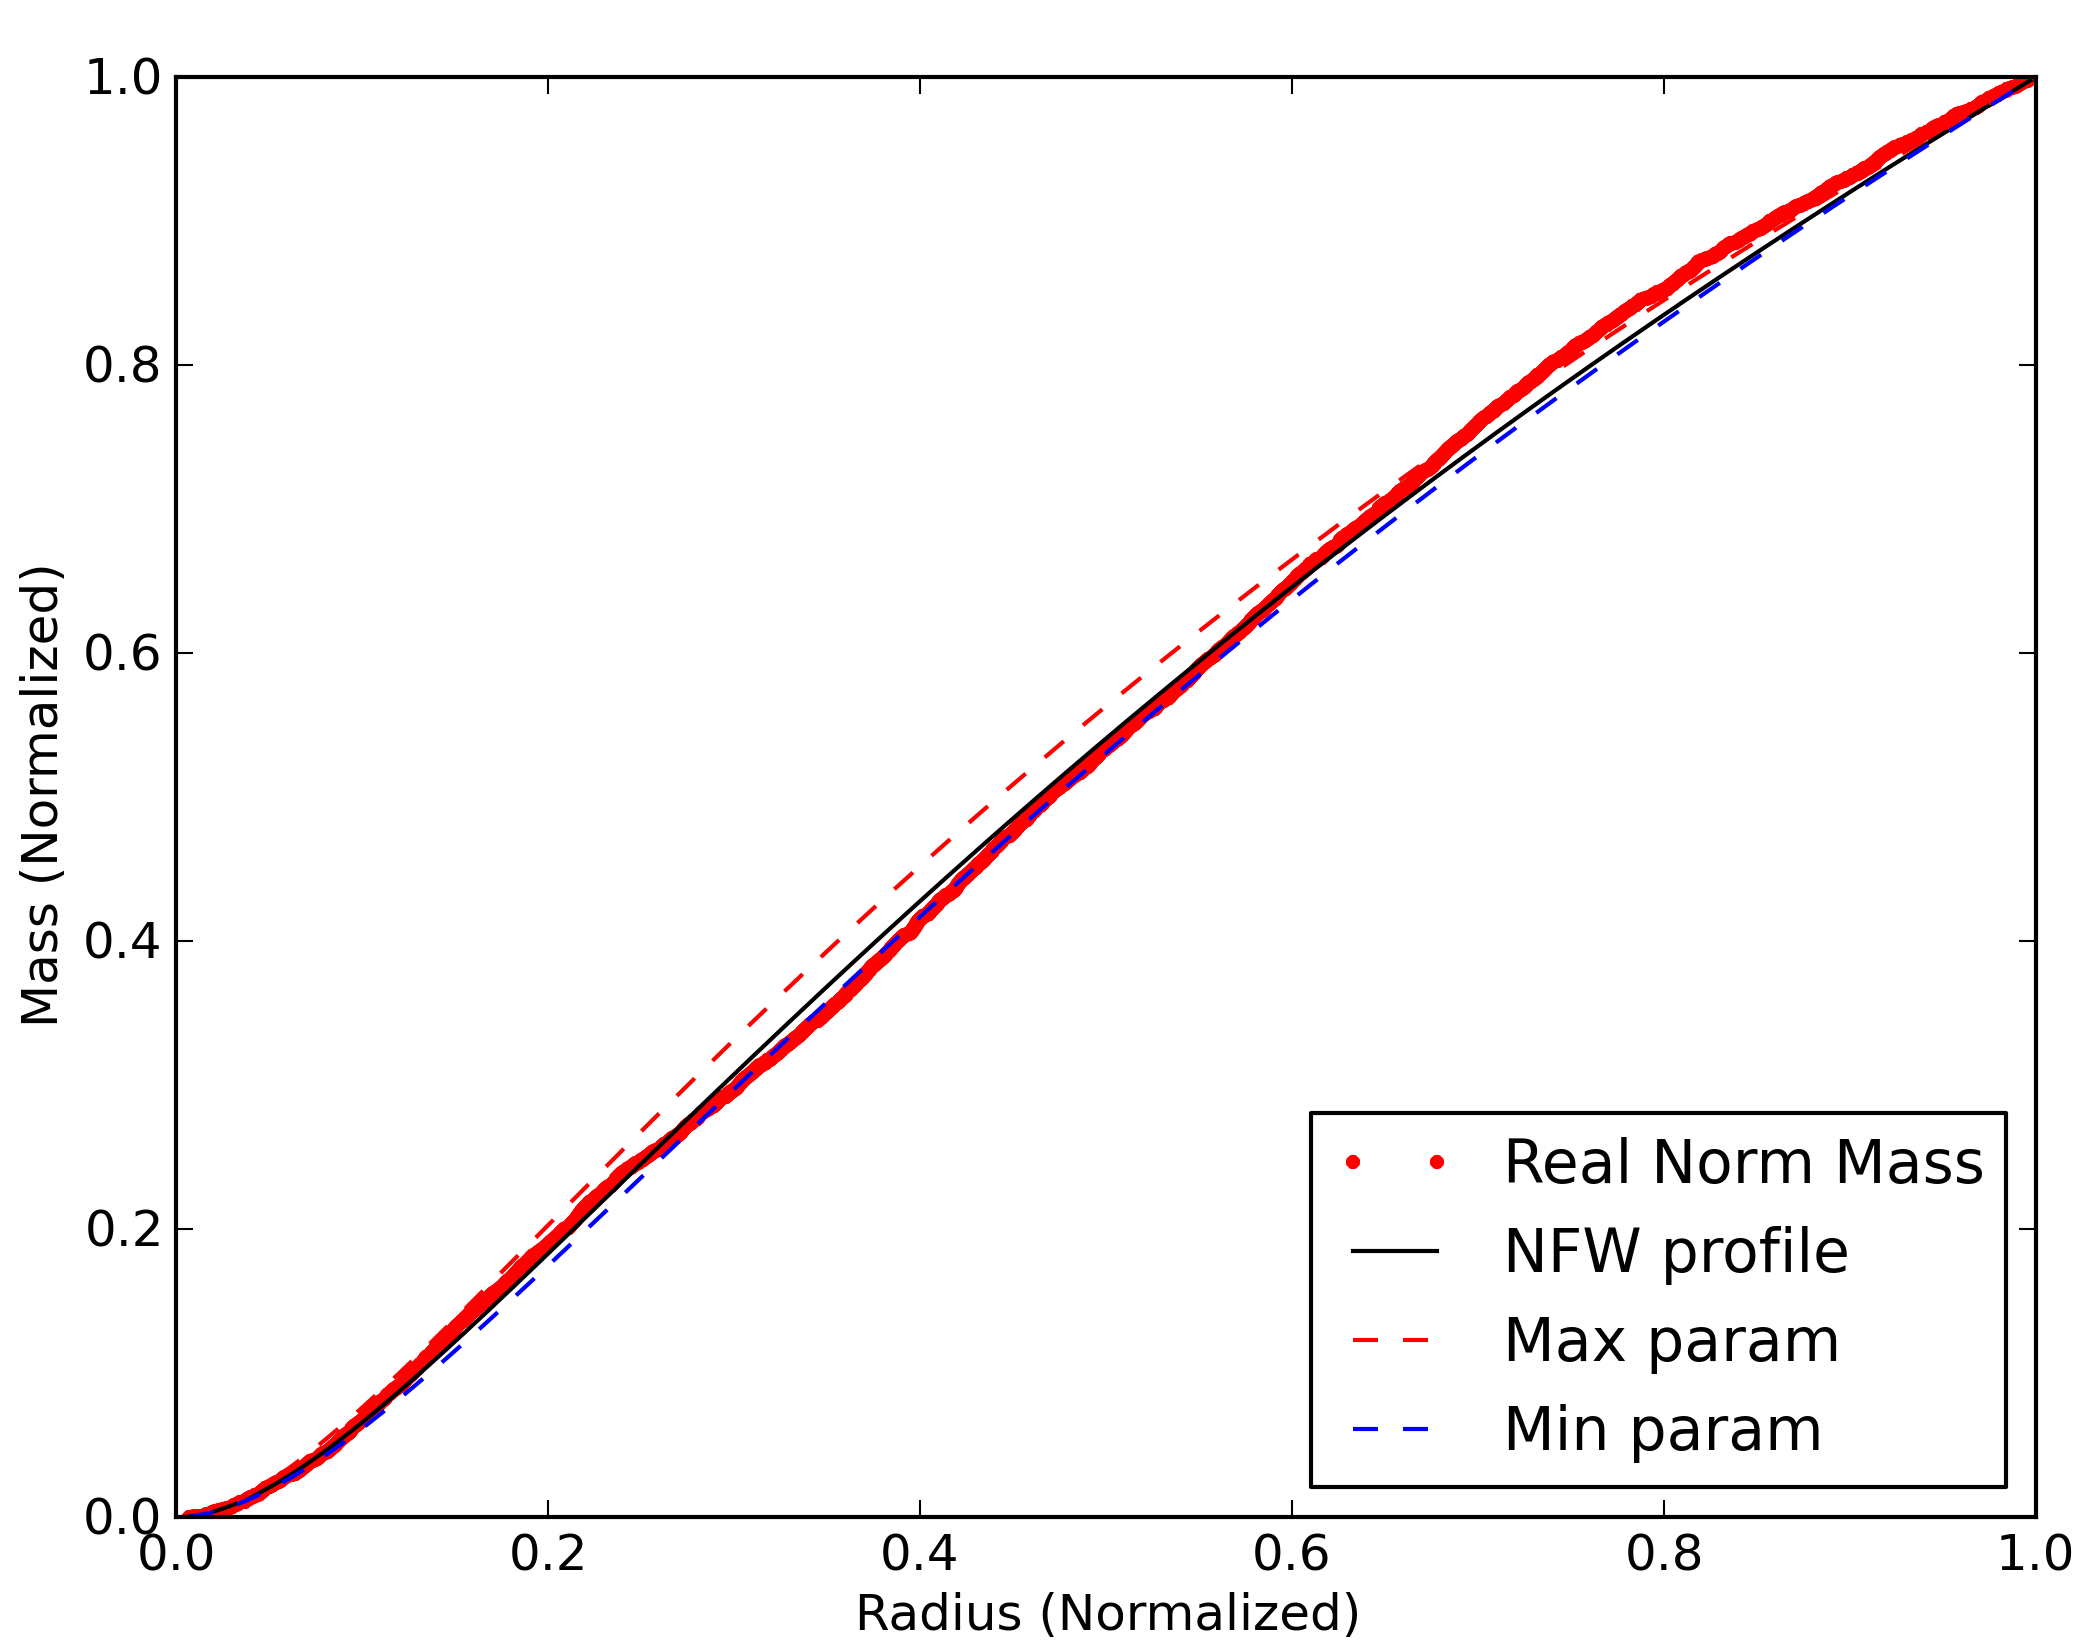
\includegraphics[scale=0.6]{mass_norm_BDMW}
\par\end{center}


\section{Resultados}

Usando los datos de la simulación MDR1\citep{MULTIDARK} se compararon
los valores de la concentración obtenidos por BDM con los obtenidos
por este método usando el catálogo FOF como base. Sin embargo no existe
una correspondecia uno a uno entre estos dos catálogos, asi que se
le asigna a cada halo de BDM un compañero en FOF como los halos con
centros más cercanos, al tomar la mediana de la concentración contra
la masa de cada halo tenemos que

\begin{center}
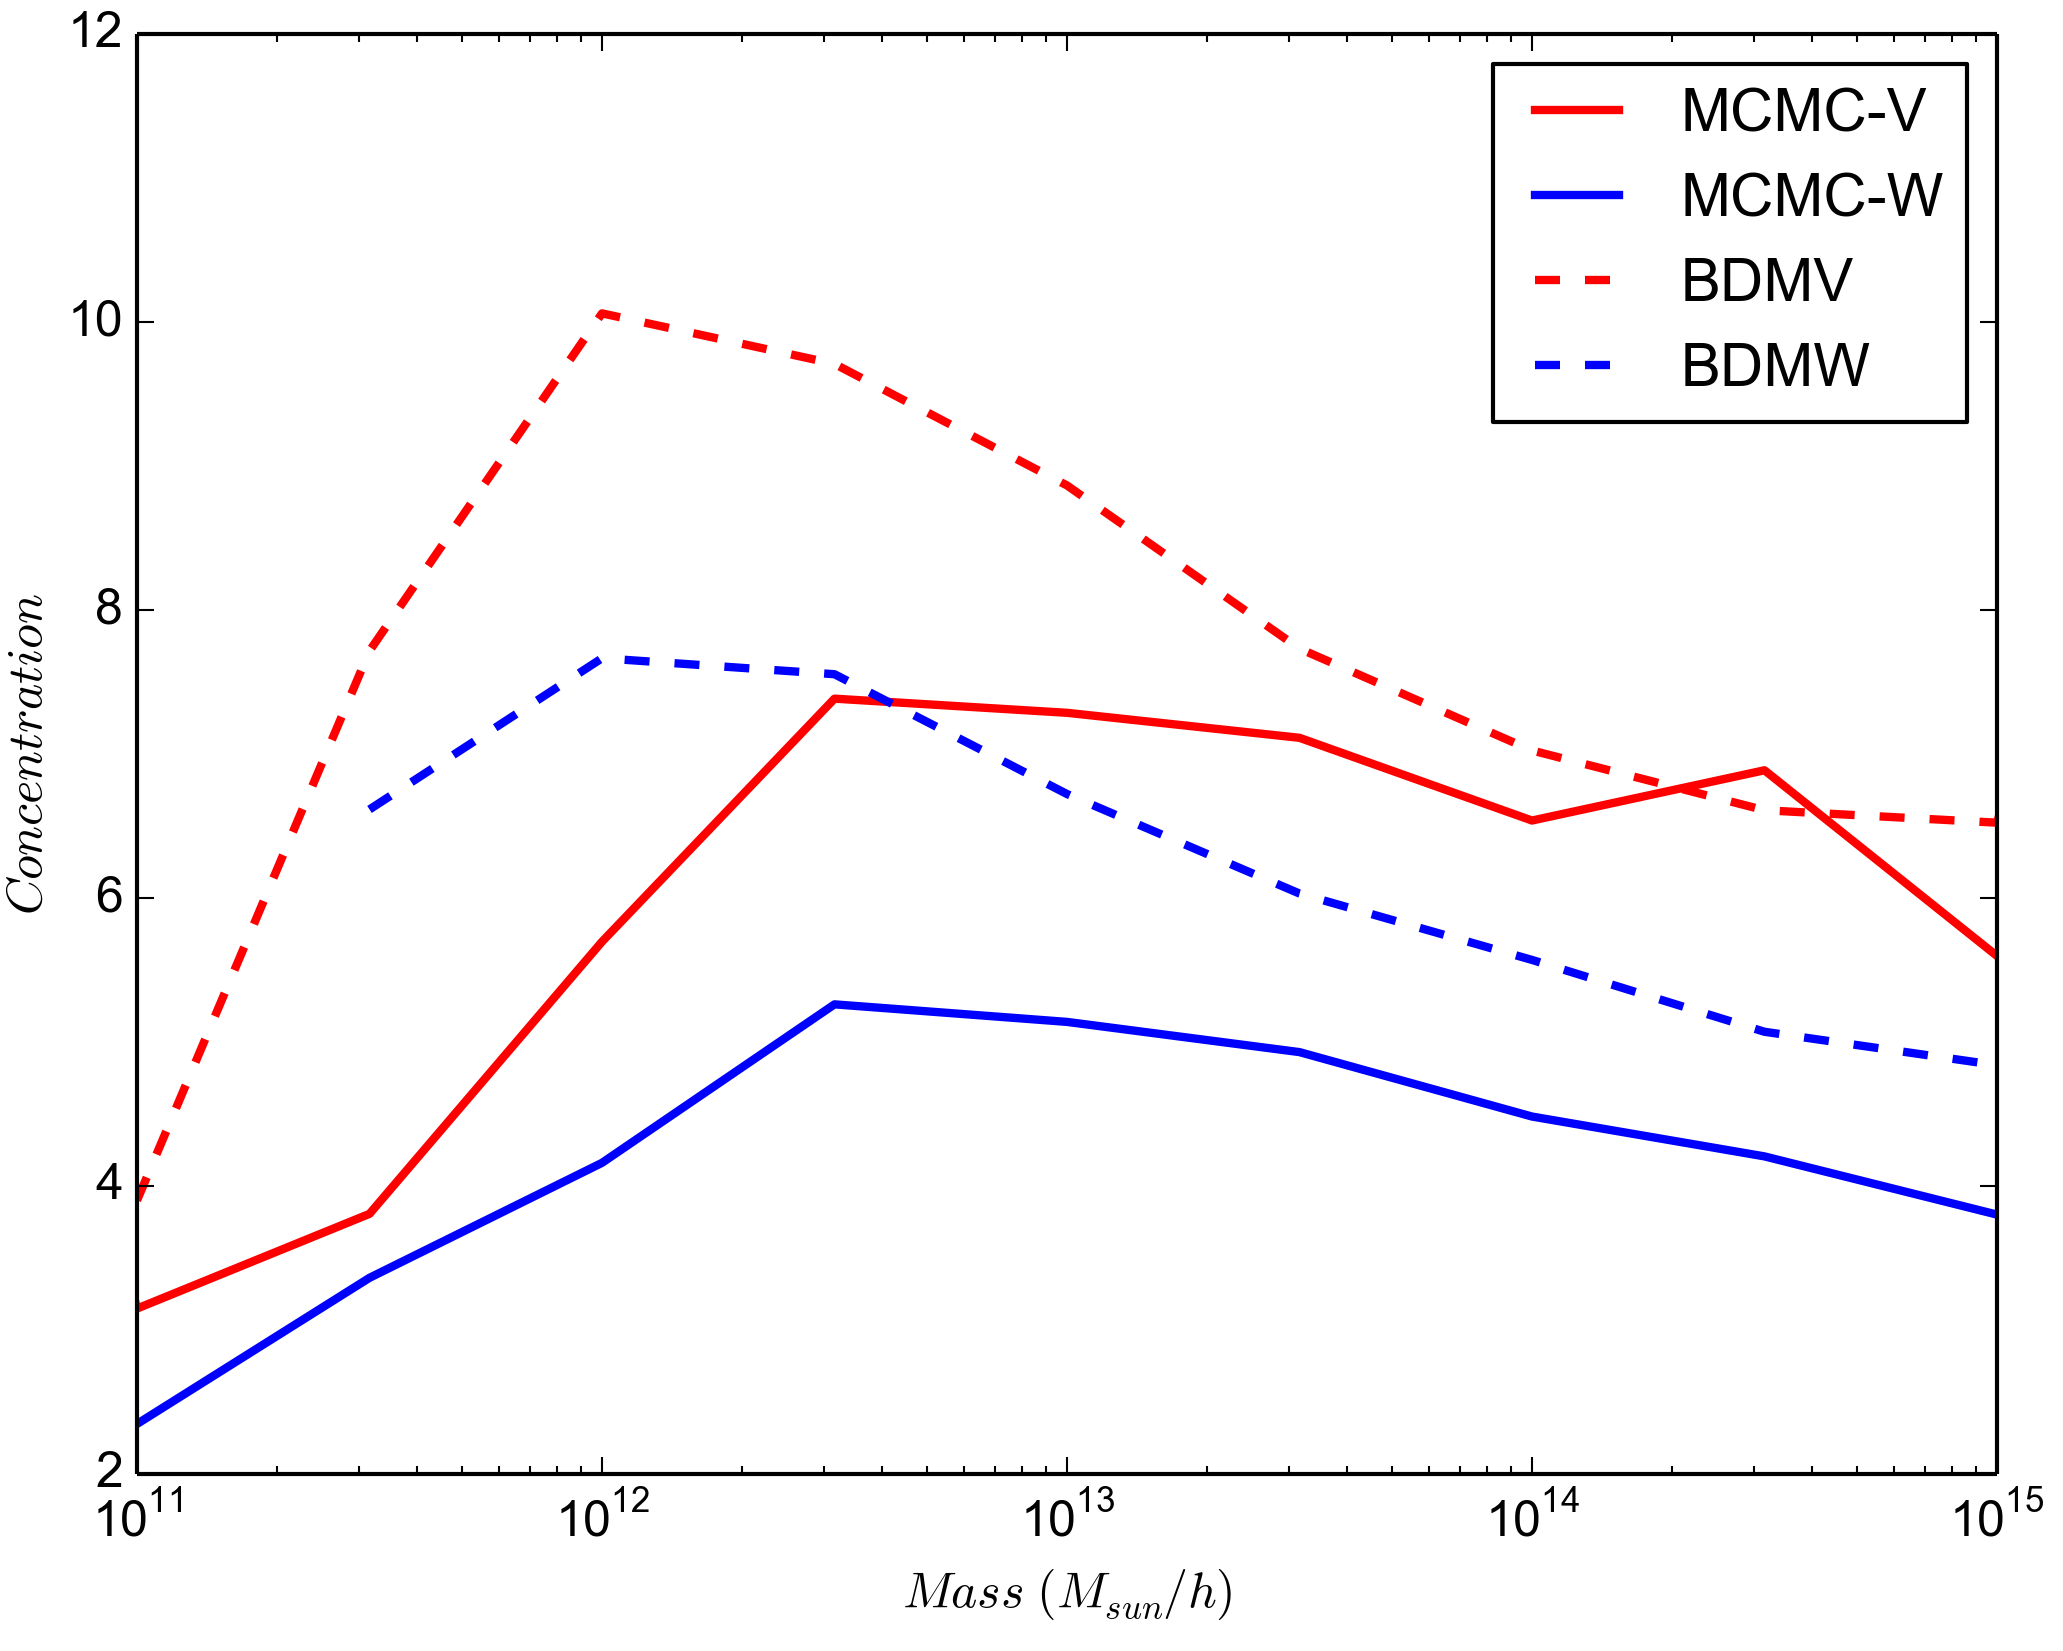
\includegraphics[scale=0.6]{concentration}
\par\end{center}


\section{Discusión}

A diferencia del estimado de la concentración dada por \emph{BDM }este
método permite obtener un estimado más directo. Sin embargo no se
sabe a que se deben las discrepancias entre los resultados obtenidos,
aun es necesario determinar si estas diferencias se deben al algorítmo
utilizado en si o a la población de datos que se tomó.
\begin{thebibliography}{1}
\bibitem{NFW}The Structure of cold dark matter halos - Navarro, Julio
F. et al. Astrophys.J. 462 (1996) 563-575 astro-ph/9508025

\bibitem{MULTIDARK}MDR1 Database. En Multidark Database (sf). Recuperado
el 6 de mayo de 2014, de http://www.multidark.org/MultiDark/Help?
page=databases/mdr1/database

\bibitem{BDM}Particle mesh code for cosmological simulations - Klypin,
Anatoly et al. astro-ph/9712217.

\bibitem{FOF}The Evolution of Large Scale Structure in a Universe
Dominated by Cold Dark Matter - Davis, Marc et al. Astrophys.J. 292
(1985) 371-394 NSF-ITP-84-129. 

\end{thebibliography}
\end{multicols} 
\end{document}
